\documentclass[11pt,a4paper]{report}
\usepackage{fontspec}
\setmainfont{TeX Gyre Termes}
\setsansfont{TeX Gyre Heros}
\setmonofont{Liberation Mono}[Scale=1.0]
\usepackage[a4paper,left=25mm,right=22mm,top=23mm,bottom=23mm,headheight=15pt]{geometry}
\usepackage{xcolor,graphicx,booktabs,longtable,tabularx,array,multirow}
\usepackage{tikz}\usetikzlibrary{arrows.meta,shapes.geometric,positioning,calc}
\usepackage{fvextra,float,caption,enumitem,titlesec,fancyhdr,lastpage,needspace,etoolbox}
\usepackage[unicode,hypertexnames=false,colorlinks=true,linkcolor=Ink,urlcolor=Accent,citecolor=Accent]{hyperref}
\definecolor{Ink}{HTML}{173453}\definecolor{Accent}{HTML}{007A9D}
\definecolor{Pale}{HTML}{EDF4F8}\definecolor{Edge}{HTML}{8AA6BB}
\definecolor{ErrorInk}{HTML}{923D44}\definecolor{Gold}{HTML}{FFF6DF}
\hypersetup{pdftitle={BTL2 Phần 1 và 2 Hệ thống quản lý quán Net},pdfauthor={L09 Nhóm 10},pdfsubject={GVHD ThS. Trần Thị Quế Nguyệt}}
\renewcommand{\contentsname}{Mục lục}\renewcommand{\listfigurename}{Danh mục hình}
\renewcommand{\figurename}{Hình}\renewcommand{\tablename}{Bảng}\renewcommand{\chaptername}{Phần}
\renewcommand{\bibname}{Tài liệu và nguồn đối chiếu}
\setcounter{tocdepth}{2}\setcounter{secnumdepth}{2}
\setlength{\parindent}{0pt}\setlength{\parskip}{5pt}\linespread{1.08}
\setlength{\emergencystretch}{2em}
\setlist[itemize]{leftmargin=5mm,itemsep=2pt,topsep=3pt}
\setlist[enumerate]{leftmargin=7mm,itemsep=2pt,topsep=3pt}
\pagestyle{fancy}\fancyhf{}\fancyhead[L]{\small\sffamily HỆ CƠ SỞ DỮ LIỆU | BTL2}
\fancyhead[R]{\small\sffamily L09 — Nhóm 10}\fancyfoot[C]{\small\thepage}
\renewcommand{\headrulewidth}{0.3pt}
\fancypagestyle{plain}{\fancyhf{}\fancyfoot[C]{\small\thepage}\renewcommand{\headrulewidth}{0pt}}
\titleformat{\chapter}[display]{\sffamily\bfseries\color{Ink}}{\large PHẦN \thechapter}{6pt}{\LARGE}
\titlespacing*{\chapter}{0pt}{-10pt}{18pt}
\titleformat{\section}{\sffamily\large\bfseries\color{Ink}}{\thesection}{.7em}{}
\titleformat{\subsection}{\sffamily\normalsize\bfseries\color{Ink}}{\thesubsection}{.7em}{}
\preto\section{\Needspace{10\baselineskip}}
\preto\subsection{\Needspace{6\baselineskip}}
\captionsetup{font=small,labelfont=bf,labelsep=period,skip=7pt}
\newcolumntype{Y}{>{\raggedright\arraybackslash}X}
\newcommand{\code}[1]{\texttt{\detokenize{#1}}}
\newcommand{\sqlinput}[2]{\par\needspace{5\baselineskip}\noindent{\small\sffamily\bfseries\color{Ink}#2}\par\vspace{-2pt}\VerbatimInput[fontsize=\fontsize{8.6}{10.7}\selectfont,breaklines=true,breakanywhere=true,numbers=left,numbersep=5pt,frame=lines,framesep=3mm,rulecolor=\color{Edge},numberblanklines=false]{#1}\par}
\newcommand{\snapshot}[3]{\begin{figure}[H]\centering\includegraphics[width=\linewidth,height=.75\textheight,keepaspectratio]{assets/dbms/#1.pdf}\caption{#2}\label{#3}\end{figure}}
\tikzset{flow/.style={font=\sffamily\fontsize{9.6}{11.8}\selectfont},start/.style={ellipse,draw=Ink,fill=Ink,text=white,align=center,minimum height=9mm,inner sep=3mm},process/.style={rectangle,rounded corners=2pt,draw=Edge,fill=Pale,align=center,text width=5.6cm,minimum height=10mm,inner sep=3mm},decision/.style={diamond,aspect=2.6,draw=Accent,fill=Gold,align=center,text width=4.1cm,inner sep=1.8mm},error/.style={rectangle,rounded corners=2pt,draw=ErrorInk,fill=ErrorInk!6,align=center,text width=4.4cm,minimum height=10mm,inner sep=3mm},arrow/.style={-{Latex[length=2mm]},draw=Ink,line width=.7pt,rounded corners=3pt}}
\newcommand{\flowfigure}[3]{\begin{figure}[H]\centering\input{#1}\caption{#2}\label{#3}\end{figure}}
\begin{document}
% !TeX root = ../main.tex
\begin{titlepage}\thispagestyle{empty}
\begin{center}
{\sffamily\fontsize{11.5}{15}\selectfont ĐẠI HỌC QUỐC GIA THÀNH PHỐ HỒ CHÍ MINH}\\[3mm]
{\sffamily\bfseries\fontsize{15}{19}\selectfont TRƯỜNG ĐẠI HỌC BÁCH KHOA}\\[10mm]

\includegraphics[width=35mm]{assets/logo_bach_khoa.png}\\[11mm]
{\sffamily\color{Ink}\fontsize{14}{18}\selectfont BÁO CÁO BÀI TẬP LỚN SỐ 2}\\[3mm]
{\sffamily\bfseries\fontsize{17}{22}\selectfont HỆ CƠ SỞ DỮ LIỆU}\\[2mm]
{\sffamily\fontsize{11}{14}\selectfont Phần 1 và Phần 2 · Học kỳ 261}\\[10mm]
{\bfseries\color{Ink}\fontsize{26}{32}\selectfont HỆ THỐNG QUẢN LÝ\\QUÁN NET}\\[12mm]
\begin{tabular}{@{}rl@{}}
\textbf{GVHD:}&\textbf{ThS. Trần Thị Quế Nguyệt}\\[3mm]
\textbf{Lớp:}&L09\\[2mm]\textbf{Nhóm:}&10
\end{tabular}\\[10mm]
{\sffamily\bfseries Sinh viên thực hiện}\\[3mm]
\renewcommand{\arraystretch}{1.25}
\begin{tabular}{@{}ll@{}}\toprule
\textbf{Họ và tên} & \textbf{MSSV}\\\midrule
Nguyễn Thành Đạt & 2410709\\
Nguyễn Minh Đạt & 2410694\\
Nguyễn Phúc Bảo Đạt & 2410696\\
Nguyễn Hữu Tây & 2413095\\
Trần Tiến Thành & 2413181\\\bottomrule
\end{tabular}
\vfill
{\sffamily Thành phố Hồ Chí Minh, tháng 11 năm 2026}
\end{center}\end{titlepage}

\pagenumbering{roman}
\tableofcontents\clearpage
\chapter*{Phạm vi và cách đọc báo cáo}\addcontentsline{toc}{chapter}{Phạm vi và cách đọc báo cáo}
Báo cáo trình bày phần hiện thực cơ sở dữ liệu của hệ thống quản lý quán Net, kế thừa mô hình 23 bảng từ BTL1. Phạm vi Phần 1–2 gồm lược đồ vật lý, dữ liệu mẫu, chỉ mục, truy vấn, thủ tục, hàm và trigger. Ứng dụng Flask được dùng để kiểm chứng các giao dịch và ba luồng vận hành liên quan.

Các câu SQL trong báo cáo lấy từ bộ mã bàn giao. Ảnh minh chứng là bản xuất trực tiếp của SQL client kết nối MySQL 8.4.13; câu lệnh và đầu ra thô được lưu theo từng lần chạy. Các lưu đồ được dựng bằng TikZ, còn sơ đồ EER được nhúng ở dạng vector để phóng to không vỡ chữ. Câu lệnh và tập kết quả chính được trình bày bằng văn bản/bảng; các hình toàn màn hình giữ vai trò đối chiếu phiên thực thi.
\begin{table}[H]\small\centering\caption{Đối chiếu cấu trúc báo cáo với mẫu Phần 1–2}
\begin{tabularx}{\linewidth}{@{}p{30mm}Yp{31mm}@{}}\toprule
\textbf{Nội dung} & \textbf{Sản phẩm trình bày} & \textbf{Vị trí}\\\midrule
Bảng và ràng buộc & 23 bảng; khóa, miền giá trị và các ca vi phạm & Mục \ref{sec:schema}\\
Chỉ mục & Lý do lựa chọn; kế hoạch và số đo trước/sau & Mục \ref{sec:index}\\
Truy vấn & Năm truy vấn, dữ liệu và kết quả đối chiếu & Mục \ref{sec:queries}\\
SQL nghiệp vụ & CRUD, hai yêu cầu trigger, hai thủ tục và hai hàm & Phần \ref{chap:routines}\\
Kiểm chứng & Ca đúng/sai, hồi quy và ba luồng demo & Phần \ref{chap:verification}\\
Phụ lục & Phân công, EER vector, dữ liệu và nguồn bàn giao & Các phụ lục\\\bottomrule
\end{tabularx}\end{table}
\clearpage\pagenumbering{arabic}
% !TeX root = ../main.tex
\chapter{Tạo bảng, dữ liệu mẫu và truy vấn dữ liệu (10đ)}\label{chap:schema}
\section{Các câu lệnh tạo bảng và ràng buộc kiểm tra (3.5đ)}\label{sec:schema}
\subsection{Tổ chức lược đồ}
Hệ thống quản lý đồng thời thời gian sử dụng máy, ví hội viên, bán dịch vụ và tồn kho. Một sự kiện kinh tế được lưu qua chứng từ: phiên và biên lai cho tiền máy; đơn cùng dòng chi tiết cho dịch vụ; phiếu cùng dòng chi tiết cho nhập, xuất hoặc kiểm kê. Cách tổ chức này giúp truy nguyên thay đổi số dư và tồn thay vì chỉ lưu các giá trị tổng hiện tại.

MySQL 8.4.13 sử dụng InnoDB để hỗ trợ khóa ngoại và giao dịch. Các mã định danh dùng so sánh nhị phân \code{ascii_bin}; dữ liệu văn bản dùng \code{utf8mb4_0900_as_cs}. Tiền VND được lưu theo số nguyên; giá trị dẫn xuất ở dòng chi tiết được tính từ số lượng và đơn giá.
\begin{table}[H]\centering\small\caption{Năm phân hệ trong lược đồ 23 bảng}
\begin{tabularx}{\linewidth}{@{}p{34mm}Yc@{}}\toprule
\textbf{Phân hệ}&\textbf{Các bảng}&\textbf{Số bảng}\\\midrule
Danh tính & NHOM\_NGUOI\_DUNG, TAI\_KHOAN, SO\_DIEN\_THOAI, NGUOI\_CHOI, NHAN\_VIEN, DIA\_CHI\_NV & 6\\
Máy trạm & KHU\_VUC, NHOM\_MAY, BANG\_GIA, MAY\_TRAM, PHIEN\_SU\_DUNG, BIEN\_LAI\_TIEN\_MAY & 6\\
Dịch vụ & NHOM\_DICH\_VU, DON\_VI\_TINH, MAY\_IN, DICH\_VU, DON\_GOI\_DICH\_VU, CHI\_TIET\_GOI\_DICH\_VU & 6\\
Kho & PHIEU\_KHO, CHI\_TIET\_PHIEU\_KHO & 2\\
Nhân sự và ví & CA\_TRUC, PHAN\_CONG\_TRUC, GIAO\_DICH\_VI & 3\\\bottomrule
\end{tabularx}\end{table}
\subsection{Câu lệnh tạo bảng}
Các tệp sau là nguồn DDL được dùng khi khởi tạo database mới. Khóa chính định danh từng thực thể; UNIQUE ngăn trùng mã nghiệp vụ; CHECK giới hạn trạng thái, miền tiền, số lượng và thứ tự thời gian. Cột sinh kết hợp UNIQUE được dùng cho các trường hợp cần đảm bảo duy nhất có điều kiện, chẳng hạn một máy chỉ có một phiên đang hoạt động.
\sqlinput{sql/01_identity.sql}{DDL phân hệ danh tính}
\sqlinput{sql/02_workstations.sql}{DDL phân hệ máy trạm}
\sqlinput{sql/03_services.sql}{DDL phân hệ dịch vụ}
\sqlinput{sql/04_inventory.sql}{DDL phân hệ kho}
\sqlinput{sql/05_staff_wallet.sql}{DDL phân hệ nhân sự và ví}
\subsection{Khóa ngoại và chính sách toàn vẹn}
Khóa ngoại bảo đảm các dòng chi tiết và chứng từ tham chiếu đối tượng tồn tại. Các tham chiếu lịch sử dùng RESTRICT khi việc xóa đối tượng cha có thể làm mất khả năng đối soát. CASCADE chỉ được sử dụng theo quan hệ đã định nghĩa trong DDL; không được hiểu là quyền tùy ý xóa chứng từ đã chốt.
\sqlinput{sql/constraints.sql}{Các khóa ngoại được áp dụng}
\snapshot{img_01_dbms_tables}{Kết quả DBMS minh họa câu lệnh tạo bảng thực thi thành công (23 bảng)}{fig:img_01_dbms_tables}
\snapshot{img_02_dbms_constraints}{Kết quả DBMS minh họa các ràng buộc khóa ngoại và CHECK được áp dụng}{fig:img_02_dbms_constraints}
\section{Câu lệnh tạo chỉ mục (1.5đ)}\label{sec:index}
\subsection{Mô tả lý do cần đánh chỉ mục}
Ở màn hình gọi món tại máy hoặc bán tại quầy, người dùng lọc dịch vụ đang kinh doanh theo nhóm và khoảng giá, sau đó xem giá từ cao xuống thấp. Yêu cầu này xuất phát từ chức năng xem thực đơn phục vụ khách và thu ngân. Truy vấn Q-P12-02 vì vậy là cơ sở lựa chọn chỉ mục nhiều cột, không đánh chỉ mục tách rời khỏi nhu cầu sử dụng thực tế.
\sqlinput{sql/indexes.sql}{Câu lệnh tạo chỉ mục: ix\_dich\_vu\_filter}
\subsection{Minh họa hiệu quả truy vấn trước và sau khi đánh chỉ mục}
Phép đo dùng database riêng với 20.000 dòng dịch vụ, 10 nhóm và hai đơn vị tính. Cùng một câu SELECT được chạy 20 lượt trước và sau khi thêm \code{ix_dich_vu_filter}. Cả hai giai đoạn đều lấy hết tập kết quả. Số đo phụ thuộc máy chạy, cache và tải tại thời điểm đo; đây là bằng chứng cho tập dữ liệu cụ thể, không phải cam kết hiệu năng trong mọi môi trường.
\begin{table}[H]\centering\caption{So sánh hiệu năng truy vấn trước và sau khi đánh chỉ mục}\begin{tabularx}{\linewidth}{@{}Yrr@{}}\toprule\textbf{Chỉ tiêu}&\textbf{Trước}&\textbf{Sau}\\\midrule
Thời gian trung bình 20 lượt (ms)&267.313&68.820\\
Số dòng kết quả&949&949\\
Có bước Sort&Có&Có\\\bottomrule\end{tabularx}\end{table}
Hiệu quả tăng tốc đạt \textbf{3.88 lần} (từ 267.3ms xuống 68.8ms). Kế hoạch thực thi dưới đây minh họa chi tiết đường dẫn truy xuất dữ liệu từ Table Scan sang Index Range Scan:
\sqlinput{sql/plan_before.txt}{Kế hoạch thực thi EXPLAIN ANALYZE trước khi tạo chỉ mục}
\sqlinput{sql/plan_after.txt}{Kế hoạch thực thi EXPLAIN ANALYZE sau khi tạo chỉ mục}
\snapshot{index_before}{Kết quả DBMS hiển thị EXPLAIN ANALYZE trước khi tạo chỉ mục}{fig:index_before}
\snapshot{index_after}{Kết quả DBMS hiển thị EXPLAIN ANALYZE sau khi tạo chỉ mục}{fig:index_after}
\section{Truy vấn dữ liệu (5đ)}\label{sec:queries}
Yêu cầu: 5 câu truy vấn độc lập trên các bảng dữ liệu khác nhau, kèm dữ liệu mẫu và kết quả thực thi trên DBMS. Hai câu đầu có SELECT, FROM, WHERE, ORDER BY; hai câu tiếp theo có GROUP BY và AGGREGATE; câu cuối cùng lồng 2 cấp và AGGREGATE. Các bảng dữ liệu mẫu chi tiết được đối chiếu thêm tại Phụ lục \ref{app:data}.
\subsection{Câu truy vấn 1: Danh sách máy theo khu vực (Q-P12-01)}
Mô tả: Dùng cho màn hình sơ đồ máy của thu ngân để kiểm tra các máy có thể sử dụng tại KV01, hiển thị tên máy, nhóm máy và đơn giá giờ; sắp xếp theo vị trí hàng, cột.
\sqlinput{sql/Q-P12-01.sql}{Câu lệnh SELECT - Truy vấn 1 (Q-P12-01)}
\begin{table}[H]
\centering\small
\caption{Bảng dữ liệu mẫu và kết quả thực thi Truy vấn 1}
\begin{tabularx}{\linewidth}{@{}XXXXX@{}}\toprule
\textbf{Mã máy} & \textbf{Tên máy} & \textbf{Trạng thái} & \textbf{Nhóm máy} & \textbf{Giá giờ}\\\midrule
M01 & Máy 01 & AVAILABLE & Máy VIP & 15000\\
M02 & Máy 02 & AVAILABLE & Máy VIP & 15000\\
M04 & Máy 04 & AVAILABLE & Máy VIP & 15000\\
\bottomrule\end{tabularx}\end{table}
\snapshot{img_04_q01}{Kết quả màn hình hiển thị từ DBMS minh họa thực thi Truy vấn 1}{fig:img_04_q01}
\subsection{Câu truy vấn 2: Lọc thực đơn theo nhóm và giá (Q-P12-02)}
Mô tả: Dùng cho màn hình gọi món của khách hoặc bán tại quầy của thu ngân để tìm các món thuộc nhóm NDV01 có giá từ 10.000 đến 50.000đ; sắp theo giá giảm dần rồi theo mã.
\sqlinput{sql/Q-P12-02.sql}{Câu lệnh SELECT - Truy vấn 2 (Q-P12-02)}
\begin{table}[H]
\centering\small
\caption{Bảng dữ liệu mẫu và kết quả thực thi Truy vấn 2}
\begin{tabularx}{\linewidth}{@{}XXXXX@{}}\toprule
\textbf{Mã DV} & \textbf{Tên dịch vụ} & \textbf{Đơn vị} & \textbf{Giá bán} & \textbf{Tồn}\\\midrule
DV03 & Cơm chiên trứng & Phần & 25000 & 30\\
DV01 & Mì trứng & Phần & 15000 & 50\\
\bottomrule\end{tabularx}\end{table}
\snapshot{img_05_q02}{Kết quả màn hình hiển thị từ DBMS minh họa thực thi Truy vấn 2}{fig:img_05_q02}
\subsection{Câu truy vấn 3: Tổng hợp đơn đã thanh toán (Q-P12-03)}
Mô tả: Dùng cho màn hình báo cáo ca của quản lý để thống kê số đơn và doanh số theo ngày đặt và kênh đặt; có nhóm theo ngày, kênh và tính tổng tiền, đếm số đơn.
\sqlinput{sql/Q-P12-03.sql}{Câu lệnh SELECT - Truy vấn 3 (Q-P12-03)}
\begin{table}[H]
\centering\small
\caption{Bảng dữ liệu mẫu và kết quả thực thi Truy vấn 3}
\begin{tabularx}{\linewidth}{@{}XXXX@{}}\toprule
\textbf{Ngày đặt} & \textbf{Kênh đặt} & \textbf{Số đơn} & \textbf{Tổng tiền}\\\midrule
2026-10-21 & TaiQuay & 1 & 50000\\
2026-10-20 & TaiQuay & 1 & 52000\\
\bottomrule\end{tabularx}\end{table}
\snapshot{img_06_q03}{Kết quả màn hình hiển thị từ DBMS minh họa thực thi Truy vấn 3}{fig:img_06_q03}
\subsection{Câu truy vấn 4: Số ca và thời lượng trực (Q-P12-04)}
Mô tả: Dùng cho màn hình chấm công và phân ca để thống kê tổng số ca và tổng thời lượng trực của nhân viên; loại bỏ trùng lặp mã ca trước khi cộng tổng.
\sqlinput{sql/Q-P12-04.sql}{Câu lệnh SELECT - Truy vấn 4 (Q-P12-04)}
\begin{table}[H]
\centering\small
\caption{Bảng dữ liệu mẫu và kết quả thực thi Truy vấn 4}
\begin{tabularx}{\linewidth}{@{}XXXX@{}}\toprule
\textbf{Mã NV} & \textbf{Tên nhân viên} & \textbf{Số ca} & \textbf{Số giờ}\\\midrule
TK07 & Demo barista & 2 & 10.00\\
TK01 & Demo admin & 1 & 5.00\\
TK03 & Demo cashier1 & 1 & 5.00\\
\bottomrule\end{tabularx}\end{table}
\snapshot{img_07_q04}{Kết quả màn hình hiển thị từ DBMS minh họa thực thi Truy vấn 4}{fig:img_07_q04}
\subsection{Câu truy vấn 5: Hội viên có số dư vượt mức trung bình (Q-P12-05)}
Mô tả: Dùng cho màn hình chăm sóc khách hàng VIP để tìm hội viên có số dư ví cao hơn mức số dư trung bình của nhóm hội viên từng phát sinh giao dịch ví thành công.
\sqlinput{sql/Q-P12-05.sql}{Câu lệnh SELECT - Truy vấn 5 (Q-P12-05)}
\begin{table}[H]
\centering\small
\caption{Bảng dữ liệu mẫu và kết quả thực thi Truy vấn 5}
\begin{tabularx}{\linewidth}{@{}XXXX@{}}\toprule
\textbf{Mã hội viên} & \textbf{Tên hội viên} & \textbf{Số dư ví} & \textbf{Ngày đăng ký}\\\midrule
TK09 & Demo player3 & 250000 & 2026-10-01\\
\bottomrule\end{tabularx}\end{table}
\snapshot{img_08_q05}{Kết quả màn hình hiển thị từ DBMS minh họa thực thi Truy vấn 5}{fig:img_08_q05}

% !TeX root = ../main.tex
\chapter{THỦ TỤC – HÀM - TRIGGER}\label{chap:routines}
\section{Thủ tục INSERT / UPDATE / DELETE dữ liệu vào 1 bảng dữ liệu}
\subsection{Nguyên tắc xử lý và bảng dữ liệu chính}
Bảng dữ liệu chính liên quan: \code{KHU_VUC}. Bảng dữ liệu phụ liên quan: \code{MAY_TRAM}, \code{PHAN_CONG_TRUC}. Thủ tục kiểm tra đầy đủ điều kiện ràng buộc nghiệp vụ và xử lý ngoại lệ có mã lỗi rõ ràng. Mỗi thủ tục trả về mã khu vực, tên thao tác và số dòng bị tác động.
\subsection{Thủ tục INSERT: Thêm khu vực (sp\_khu\_vuc\_insert)}
Mô tả: Thêm khu vực mới trong màn hình quản trị mặt bằng quán. Kiểm tra mã không rỗng, tên không trùng. Input: \code{p_ma_khu_vuc}, \code{p_ten_khu_vuc}, \code{p_mo_ta_vi_tri}. Output: \code{ma_khu_vuc}, \code{thao_tac}, \code{so_dong_tac_dong}.
\flowfigure{diagrams/crud_insert.tex}{Lưu đồ minh họa thao tác xử lý thủ tục INSERT}{fig:flow-crud_insert}
\sqlinput{sql/insert.sql}{Câu lệnh tạo thủ tục INSERT}
\sqlinput{sql/demo_img_09_crud_insert.sql}{Câu lệnh kiểm chứng trên MySQL}
\snapshot{img_09_crud_insert}{Kết quả từ DBMS minh họa kiểm tra thủ tục INSERT (trường hợp báo lỗi và trường hợp đúng)}{fig:img_09_crud_insert}
\subsection{Thủ tục UPDATE: Cập nhật khu vực (sp\_khu\_vuc\_update)}
Mô tả: Cập nhật thông tin tên và vị trí khu vực. Kiểm tra khu vực tồn tại, tên mới không trùng khu vực khác. Input: \code{p_ma_khu_vuc}, \code{p_ten_moi}, \code{p_mo_ta_moi}. Output: \code{ma_khu_vuc}, \code{thao_tac}, \code{so_dong_tac_dong}.
\flowfigure{diagrams/crud_update.tex}{Lưu đồ minh họa thao tác xử lý thủ tục UPDATE}{fig:flow-crud_update}
\sqlinput{sql/update.sql}{Câu lệnh tạo thủ tục UPDATE}
\sqlinput{sql/demo_img_10_crud_update.sql}{Câu lệnh kiểm chứng trên MySQL}
\snapshot{img_10_crud_update}{Kết quả từ DBMS minh họa kiểm tra thủ tục UPDATE (trường hợp báo lỗi và trường hợp đúng)}{fig:img_10_crud_update}
\subsection{Thủ tục DELETE: Xóa khu vực (sp\_khu\_vuc\_delete)}
Mô tả: Xóa khu vực không còn hoạt động. Kiểm tra khu vực tồn tại và không còn máy trạm hoặc lịch trực tham chiếu. Input: \code{p_ma_khu_vuc}. Output: \code{ma_khu_vuc}, \code{thao_tac}, \code{so_dong_tac_dong}.
\flowfigure{diagrams/crud_delete.tex}{Lưu đồ minh họa thao tác xử lý thủ tục DELETE}{fig:flow-crud_delete}
\sqlinput{sql/delete.sql}{Câu lệnh tạo thủ tục DELETE}
\sqlinput{sql/demo_img_11_crud_delete.sql}{Câu lệnh kiểm chứng trên MySQL}
\snapshot{img_11_crud_delete}{Kết quả từ DBMS minh họa kiểm tra thủ tục DELETE (trường hợp báo lỗi và trường hợp đúng)}{fig:img_11_crud_delete}
\snapshot{routines_created}{Kết quả màn hình hiển thị từ DBMS minh họa cho việc tạo các thủ tục CRUD}{fig:routines_created}
\section{TRIGGER}
\subsection{Trigger 1: Bảo vệ biên lai đã thanh toán (T-P12-01)}
Bảng dữ liệu chính liên quan: \code{BIEN_LAI_TIEN_MAY}. Mô tả: Trigger kiểm tra ràng buộc nghiệp vụ kế toán — không cho phép sửa đổi hoặc xóa biên lai đã ở trạng thái thanh toán (\code{DA_THANH_TOAN}). Được kích hoạt BEFORE UPDATE và BEFORE DELETE. Vẽ flowchart minh họa xử lý.
\flowfigure{diagrams/receipt.tex}{Lưu đồ minh họa xử lý Trigger 1 bảo vệ biên lai đã thanh toán}{fig:flow-receipt}
\sqlinput{sql/trigger_receipt.sql}{Câu lệnh tạo Trigger 1 trên BIEN\_LAI\_TIEN\_MAY}
\sqlinput{sql/demo_img_12_trigger_t1.sql}{Câu lệnh kiểm chứng trên MySQL}
\snapshot{img_12_trigger_t1}{Kết quả DBMS minh họa trường hợp báo lỗi: Chặn sửa và xóa biên lai đã thanh toán}{fig:img_12_trigger_t1}
\sqlinput{sql/demo_trigger_t1_valid.sql}{Câu lệnh kiểm chứng trên MySQL}
\snapshot{trigger_t1_valid}{Kết quả DBMS minh họa trường hợp đúng: Cho phép sửa và xóa biên lai chưa thanh toán}{fig:trigger_t1_valid}
\subsection{Trigger 2: Đồng bộ tổng tiền đơn từ chi tiết (T-P12-02)}
Bảng dữ liệu chính liên quan: \code{CHI_TIET_GOI_DICH_VU}. Bảng dữ liệu phụ liên quan: \code{DON_GOI_DICH_VU}. Mô tả: Nhóm trigger thao tác ảnh hưởng tới hơn 1 bảng — tự động cập nhật tổng tiền đầu đơn (\code{tong_tien}) khi thêm, sửa số lượng/giá, hoặc xóa dòng chi tiết món. Kích hoạt AFTER INSERT, AFTER UPDATE, AFTER DELETE.
\flowfigure{diagrams/order_total.tex}{Lưu đồ minh họa xử lý Trigger 2 đồng bộ tổng giá trị đơn hàng}{fig:flow-order_total}
\sqlinput{sql/trigger_total.sql}{Câu lệnh tạo nhóm Trigger 2 trên CHI\_TIET\_GOI\_DICH\_VU}
\sqlinput{sql/demo_trigger_t2_before.sql}{Câu lệnh kiểm chứng trên MySQL}
\snapshot{trigger_t2_before}{Dữ liệu đơn hàng ban đầu có tổng tiền bằng 0}{fig:trigger_t2_before}
\sqlinput{sql/demo_img_13_trigger_t2.sql}{Câu lệnh kiểm chứng trên MySQL}
\snapshot{img_13_trigger_t2}{Kết quả DBMS minh họa trường hợp đúng: Tổng tiền tự động đồng bộ khi thêm/sửa/xóa dòng món}{fig:img_13_trigger_t2}
\sqlinput{sql/demo_trigger_t2_errors.sql}{Câu lệnh kiểm chứng trên MySQL}
\snapshot{trigger_t2_errors}{Kết quả DBMS minh họa trường hợp báo lỗi: Chặn thao tác trên đơn đã đóng hoặc đã hủy}{fig:trigger_t2_errors}
\snapshot{triggers_created}{Các trigger trong hai yêu cầu đã được tạo}{fig:triggers_created}
\section{THỦ TỤC}
\subsection{Thủ tục 1: Báo cáo doanh thu theo ngày (sp\_bao\_cao\_doanh\_thu\_ngay)}
Mô tả thủ tục: Tổng hợp dữ liệu từ nhiều bảng (\code{BIEN_LAI_TIEN_MAY}, \code{DON_GOI_DICH_VU}). Sử dụng câu lệnh điều kiện IF kiểm tra ngày hợp lệ và vòng lặp WHILE duyệt qua từng ngày trong khoảng thời gian để tính tổng thu máy, thu dịch vụ và hoàn tiền. Output: Mảng JSON doanh thu chi tiết từng ngày.
\flowfigure{diagrams/revenue.tex}{Lưu đồ minh họa Thủ tục 1 duyệt vòng lặp WHILE tính doanh thu theo ngày}{fig:flow-revenue}
\sqlinput{sql/report_revenue.sql}{Câu lệnh tạo Thủ tục 1: sp\_bao\_cao\_doanh\_thu\_ngay}
\sqlinput{sql/demo_img_14_sp_doanh_thu.sql}{Câu lệnh kiểm chứng trên MySQL}
\snapshot{img_14_sp_doanh_thu}{Kết quả DBMS minh họa kiểm tra Thủ tục 1 (ca báo lỗi ngày sai và ca đúng trả mảng JSON)}{fig:img_14_sp_doanh_thu}
\subsection{Thủ tục 2: Báo cáo tồn và phân loại dịch vụ (sp\_bao\_cao\_ton\_dich\_vu)}
Mô tả thủ tục: Đọc dữ liệu từ bảng \code{DICH_VU}, \code{NHOM_DICH_VU}, \code{DON_VI_TINH}. Sử dụng CURSOR duyệt danh sách món kết hợp IF/ELSE phân loại trạng thái tồn kho (\code{HetHang}, \code{SapHet}, \code{DuHang}) theo ngưỡng chỉ định. Output: Mảng JSON danh sách dịch vụ và trạng thái phân loại.
\flowfigure{diagrams/stock.tex}{Lưu đồ minh họa Thủ tục 2 sử dụng CURSOR và IF phân loại tồn kho}{fig:flow-stock}
\sqlinput{sql/report_stock.sql}{Câu lệnh tạo Thủ tục 2: sp\_bao\_cao\_ton\_dich\_vu}
\sqlinput{sql/demo_img_15_sp_ton_kho.sql}{Câu lệnh kiểm chứng trên MySQL}
\snapshot{img_15_sp_ton_kho}{Kết quả DBMS minh họa kiểm tra Thủ tục 2 (ca báo lỗi ngưỡng âm và ca đúng trả dữ liệu)}{fig:img_15_sp_ton_kho}
\section{HÀM}
\subsection{Hàm 1: Tổng chi ví ròng (fn\_tong\_chi\_vi\_rong)}
Mô tả hàm: Đọc dữ liệu từ bảng \code{GIAO_DICH_VI} và \code{NGUOI_CHOI}. Sử dụng CURSOR duyệt qua lịch sử giao dịch kết hợp câu lệnh IF kiểm tra loại giao dịch (\code{TruTienMay}, \code{TruTienDichVu}, \code{HoanTien}) để tính tổng số tiền chi ròng của hội viên trong một khoảng thời gian. Input: \code{p_ma_nguoi_choi}, \code{p_tu_gio}, \code{p_den_gio}. Output: DECIMAL(18,0).
\flowfigure{diagrams/wallet.tex}{Lưu đồ minh họa Hàm 1 dùng CURSOR và IF tính tổng chi ròng}{fig:flow-wallet}
\sqlinput{sql/fn_wallet.sql}{Câu lệnh tạo Hàm 1: fn\_tong\_chi\_vi\_rong}
\sqlinput{sql/demo_img_16_fn_chi_vi.sql}{Câu lệnh kiểm chứng trên MySQL}
\snapshot{img_16_fn_chi_vi}{Kết quả DBMS minh họa kiểm tra Hàm 1 (ca đúng trả tổng tiền và ca sai mã trả NULL)}{fig:img_16_fn_chi_vi}
\subsection{Hàm 2: Tổng tiền từ dòng chi tiết đơn (fn\_tong\_tien\_don)}
Mô tả hàm: Đọc dữ liệu từ bảng \code{CHI_TIET_GOI_DICH_VU}. Sử dụng CURSOR duyệt từng dòng chi tiết của đơn hàng kết hợp kiểm tra IF điều kiện số lượng và đơn giá hợp lệ, sau đó cộng dồn thành tiền của toàn bộ đơn. Input: \code{p_ma_don_goi}. Output: DECIMAL(18,0).
\flowfigure{diagrams/order.tex}{Lưu đồ minh họa Hàm 2 dùng CURSOR tính tổng tiền đơn hàng}{fig:flow-order}
\sqlinput{sql/fn_order.sql}{Câu lệnh tạo Hàm 2: fn\_tong\_tien\_don}
\sqlinput{sql/demo_img_17_fn_tien_don.sql}{Câu lệnh kiểm chứng trên MySQL}
\snapshot{img_17_fn_tien_don}{Kết quả DBMS minh họa kiểm tra Hàm 2 (ca đúng trả tổng tiền và ca sai mã trả NULL)}{fig:img_17_fn_tien_don}

\chapter{Kiểm chứng và tích hợp ứng dụng}\label{chap:verification}
\section{Kiến trúc và giao dịch}
Giao diện HTML/CSS/JavaScript gọi REST API Flask trên cùng origin. Backend tách tuyến HTTP, dịch vụ nghiệp vụ và lớp truy cập dữ liệu. Dịch vụ nắm ranh giới BEGIN/COMMIT/ROLLBACK trên một kết nối; routine được gọi trong giao dịch đó, không tự chốt độc lập. Runtime dùng tài khoản hạn quyền, không cấp trực tiếp quyền cập nhật số dư ví hoặc tồn kho.

\flowfigure{diagrams/architecture.tex}{Luồng giao tiếp giữa giao diện, backend và MySQL}{fig:architecture}

Xác thực dùng phiên đăng nhập và kiểm tra CSRF cho API ghi. Dữ liệu đầu vào bị kiểm tra miền kiểu và phạm vi; mã yêu cầu được dùng để phân biệt gửi lặp với xung đột nội dung. Khi có tranh chấp, dữ liệu được đọc lại dưới khóa thay vì tin vào trạng thái đã đọc trước giao dịch.
\section{Ba luồng kiểm chứng}
\begin{enumerate}
\item \textbf{Phiên chơi:} chọn máy, mở phiên, kết thúc, đối chiếu biên lai và giải phóng máy. Với trả trước, giờ sử dụng và số dư khả dụng được kiểm soát tại server.
\item \textbf{Ví và dịch vụ:} nạp ví, gửi lại cùng mã, tạo/tiếp nhận/thanh toán đơn, đối chiếu số dư và tồn. Thanh toán đơn của phiên cũ vẫn phải tính tiền giữ chỗ của phiên đang hoạt động.
\item \textbf{Kho và báo cáo:} phiếu nháp không đổi tồn; ghi sổ chỉ tác động một lần; xem báo cáo với khoảng ngày chứa dữ liệu phát sinh.
\end{enumerate}
\section{Tổng hợp bộ kiểm thử}
\begin{table}[H]\centering\caption{Kết quả kiểm chứng được lưu trong hồ sơ nghiệm thu}
\begin{tabularx}{\linewidth}{@{}Yr@{}}\toprule\textbf{Nhóm ca}&\textbf{PASS}\\\midrule
API: quyền, đầu vào, chống lặp &30\\
Integration: rollback, retry, khóa và tranh chấp &45\\
SQL P1–2 &14\\
E2E HTTP và Chrome ba luồng &4\\
Ba ca hồi quy bổ sung &3\\\midrule
\textbf{Tổng; không FAIL, ERROR hoặc SKIP}&\textbf{96}\\\bottomrule
\end{tabularx}\end{table}
Đây là kết quả của bộ ca đã triển khai, không phải khẳng định mọi trạng thái có thể có đều được bao phủ. Dữ liệu test và tài khoản test được tạo riêng rồi dọn sau từng ca; không reset database ứng dụng. JUnit và log gốc nằm trong \path{evidence/final_verification/}.
\subsection{Các ca biên có ảnh hưởng trực tiếp đến tính đúng}
\begin{itemize}
\item Đơn đặt, thanh toán và hoàn ở ba ngày khác nhau được phân bổ đúng mốc thu/hoàn.
\item Ví 100.000đ đang giữ 90.000đ cho phiên mới không được trả đơn cũ 15.000đ.
\item Đơn tổng 10 tỷ và tên dịch vụ 90 ký tự không bị tràn/cắt trong hai routine liên quan.
\item Gửi lại phiếu kho khác loại trả 409; page quá lớn trả 422, không thành lỗi 500.
\end{itemize}
\section{Cài mới và đối chiếu từ gói bàn giao}
Bộ cài từ bản ZIP đã được chạy trên database/user mới: tạo 23 bảng, nạp hai đơn seed P1–2, mở giao diện và đăng nhập thành công. Chạy seed lại giữ nguyên dữ liệu; bộ seed một phần bị từ chối để tránh ghi đè không rõ trạng thái.

Các bước vận hành: cài thư viện đã khóa phiên bản, chạy script demo để sinh cấu hình riêng và khởi động MySQL/Flask, sau đó sử dụng tài khoản demo. Mật khẩu quản trị không được đưa vào báo cáo hay ZIP. Hướng dẫn đầy đủ ở README và runbook; kết quả phép thử từ ZIP ở \path{evidence/final_verification/zip_smoke.json}.
\section{Phạm vi chưa đưa vào demo}
Ứng dụng hiện minh họa ba luồng trên, chưa khóa máy vật lý. API chưa bao gồm đầy đủ hủy/hoàn, quản trị tài khoản, danh mục và ca trực. Các thao tác SQL quản trị ngoài API cần được đối chiếu riêng với toàn bộ quy tắc BTL1. Phần trình bày ứng dụng theo đợt riêng của môn học cần tuân thủ yêu cầu của đợt đó; báo cáo này tập trung vào Phần 1–2.

\appendix
% !TeX root = ../main.tex
\chapter{BẢNG KÊ NHIỆM VỤ VÀ ĐÁNH GIÁ}
\section{Bảng kê nhiệm vụ}
Bảng dưới kế thừa phân công đang lưu trong hồ sơ nhóm. Mỗi hàng chỉ đánh dấu một người phụ trách chính; nội dung tích hợp có thể được kiểm tra chéo. Các cột dùng bốn số cuối MSSV để tránh thu hẹp cột mô tả. Tỉ lệ đóng góp là mức đề xuất, không phải điểm đã được giảng viên xác nhận.
\begin{table}[H]\small\centering\caption{Danh sách thành viên và tỷ lệ điểm đề xuất}
\begin{tabularx}{\linewidth}{@{}lYc@{}}\toprule\textbf{MSSV}&\textbf{Họ và tên}&\textbf{Đề xuất}\\\midrule
2410709&Nguyễn Thành Đạt&20\%\\2410694&Nguyễn Minh Đạt&20\%\\2410696&Nguyễn Phúc Bảo Đạt&20\%\\2413095&Nguyễn Hữu Tây&20\%\\2413181&Trần Tiến Thành&20\%\\\bottomrule\end{tabularx}\end{table}
\begingroup\small\setlength{\tabcolsep}{3pt}\renewcommand{\arraystretch}{1.15}
\begin{longtable}{@{}>{\raggedright\arraybackslash}p{82mm}ccccc@{}}\caption{Bảng kê người phụ trách từng nội dung}\\\toprule
\textbf{Nội dung} &\textbf{0694}&\textbf{0696}&\textbf{3095}&\textbf{0709}&\textbf{3181}\\\midrule\endfirsthead
\toprule\textbf{Nội dung (tiếp)} &\textbf{0694}&\textbf{0696}&\textbf{3095}&\textbf{0709}&\textbf{3181}\\\midrule\endhead
\bottomrule\endfoot
Tạo bảng dữ liệu phần 1: 12 bảng danh tính và máy trạm & x &  &  &  & \\
Tạo bảng dữ liệu phần 2: 11 bảng dịch vụ, kho, ca trực và ví &  &  & x &  & \\
Tạo các ràng buộc khóa chính, duy nhất và miền giá trị (CHECK) & x &  &  &  & \\
Tạo các ràng buộc khóa ngoại bảo toàn toàn vẹn tham chiếu &  &  & x &  & \\
Demo kiểm tra tạo bảng, ràng buộc và kiểm đếm 23 bảng thành công & x &  &  &  & \\
Tạo chỉ mục phần 1: ix\_dich\_vu\_filter tăng tốc lọc thực đơn &  &  &  &  & x\\
Tạo chỉ mục phần 2 cho các bảng vận hành &  & x &  &  & \\
Đo lường hiệu năng chỉ mục trước và sau bằng EXPLAIN ANALYZE &  &  &  &  & x\\
Câu truy vấn 1 (Q-P12-01) - Bảng liên quan: MAY\_TRAM, KHU\_VUC & x &  &  &  & \\
Câu truy vấn 2 (Q-P12-02) - Bảng liên quan: DICH\_VU, NHOM\_DICH\_VU &  & x &  &  & \\
Câu truy vấn 3 (Q-P12-03) - Bảng liên quan: DON\_GOI\_DICH\_VU &  & x &  &  & \\
Câu truy vấn 4 (Q-P12-04) - Bảng liên quan: CA\_TRUC, PHAN\_CONG\_TRUC &  &  &  &  & x\\
Câu truy vấn 5 (Q-P12-05) - Bảng liên quan: NGUOI\_CHOI, GIAO\_DICH\_VI &  &  & x &  & \\
Thủ tục INSERT (sp\_khu\_vuc\_insert) - Bảng: KHU\_VUC & x &  &  &  & \\
Thủ tục UPDATE (sp\_khu\_vuc\_update) - Bảng: KHU\_VUC & x &  &  &  & \\
Thủ tục DELETE (sp\_khu\_vuc\_delete) - Bảng: KHU\_VUC & x &  &  &  & \\
Demo kiểm tra ba thủ tục CRUD khu vực với các ca đúng và lỗi & x &  &  &  & \\
Trigger 1 (T-P12-01) - Bảng: BIEN\_LAI\_TIEN\_MAY &  &  & x &  & \\
Demo kiểm tra Trigger 1 chặn sửa/xóa biên lai đã thanh toán &  &  & x &  & \\
Trigger 2 (T-P12-02) - Bảng: CHI\_TIET\_GOI\_DICH\_VU, DON\_GOI\_DICH\_VU &  &  &  & x & \\
Demo kiểm tra Trigger 2 duy trì tổng tiền đầu đơn từ chi tiết &  &  &  & x & \\
Thủ tục 1 (sp\_bao\_cao\_doanh\_thu\_ngay) - Bảng: BIEN\_LAI, DON\_GOI &  & x &  &  & \\
Demo kiểm tra Thủ tục 1 tổng hợp doanh thu theo ngày &  & x &  &  & \\
Thủ tục 2 (sp\_bao\_cao\_ton\_dich\_vu) - Bảng: DICH\_VU, NHOM\_DICH\_VU &  &  &  &  & x\\
Demo kiểm tra Thủ tục 2 phân loại tồn kho bằng CURSOR và IF &  &  &  &  & x\\
Hàm 1 (fn\_tong\_chi\_vi\_rong) - Bảng: GIAO\_DICH\_VI, NGUOI\_CHOI &  &  & x &  & \\
Demo kiểm tra Hàm 1 tính tổng chi ví ròng &  &  & x &  & \\
Hàm 2 (fn\_tong\_tien\_don) - Bảng: CHI\_TIET\_GOI\_DICH\_VU &  &  &  & x & \\
Demo kiểm tra Hàm 2 tính tổng tiền đơn hàng &  &  &  & x & \\
Kiến trúc tích hợp Backend Flask và Test suite tự động 79 ca &  &  &  & x & \\
Thiết kế sơ đồ giải thuật lưu đồ TikZ cho toàn bộ Routine & x &  &  &  & \\
Kịch bản dữ liệu và benchmark đo lường chỉ mục &  & x &  &  & \\
\end{longtable}\endgroup
\clearpage\section{Đánh giá của giáo viên}
(Điền danh sách thành viên và \% đóng góp bên dưới và để trống các cột còn lại)
\begin{table}[H]\centering\small\renewcommand{\arraystretch}{2.2}
\begin{tabularx}{\linewidth}{@{}>{\raggedright\arraybackslash}p{36mm}lp{12mm}Y>{\raggedright\arraybackslash}p{13mm}p{13mm}@{}}\toprule
\textbf{Họ tên}&\textbf{MSSV}&\textbf{Đề xuất}&\textbf{Nhận xét}&\textbf{Điểm trừ/cộng}&\textbf{Tổng}\\\midrule
Nguyễn Thành Đạt&2410709&20\%&&&\\
Nguyễn Minh Đạt&2410694&20\%&&&\\
Nguyễn Phúc Bảo Đạt&2410696&20\%&&&\\
Nguyễn Hữu Tây&2413095&20\%&&&\\
Trần Tiến Thành&2413181&20\%&&&\\\bottomrule
\end{tabularx}\end{table}
\chapter{PHỤ LỤC: Thiết kế ERD cập nhật mới nhất}\label{app:eer}
\section{Sơ đồ tổng thể EER dạng vector}
Sơ đồ tuân thủ chặt chẽ ký hiệu Chen chuẩn (thực thể hình chữ nhật, mối quan hệ hình thoi, thuộc tính hình elip, khóa chính gạch chân, thực thể và liên kết yếu nét đôi, thuộc tính đa trị nét đôi, thuộc tính dẫn xuất nét đứt, tham gia toàn phần nét đôi), được đồng bộ lại theo phong cách đơn sắc đen trắng rõ nét. Sơ đồ bao quát toàn bộ 18 thực thể và tất cả các mối quan hệ nghiệp vụ của hệ thống 23 bảng. Tệp PDF/SVG nguồn vector được lưu tại \path{assets/eer/erd_full_vector.pdf} và mô hình chỉnh sửa tại \path{docs/btl1_baseline/BTL1_EER.drawio}.
\begin{figure}[H]\centering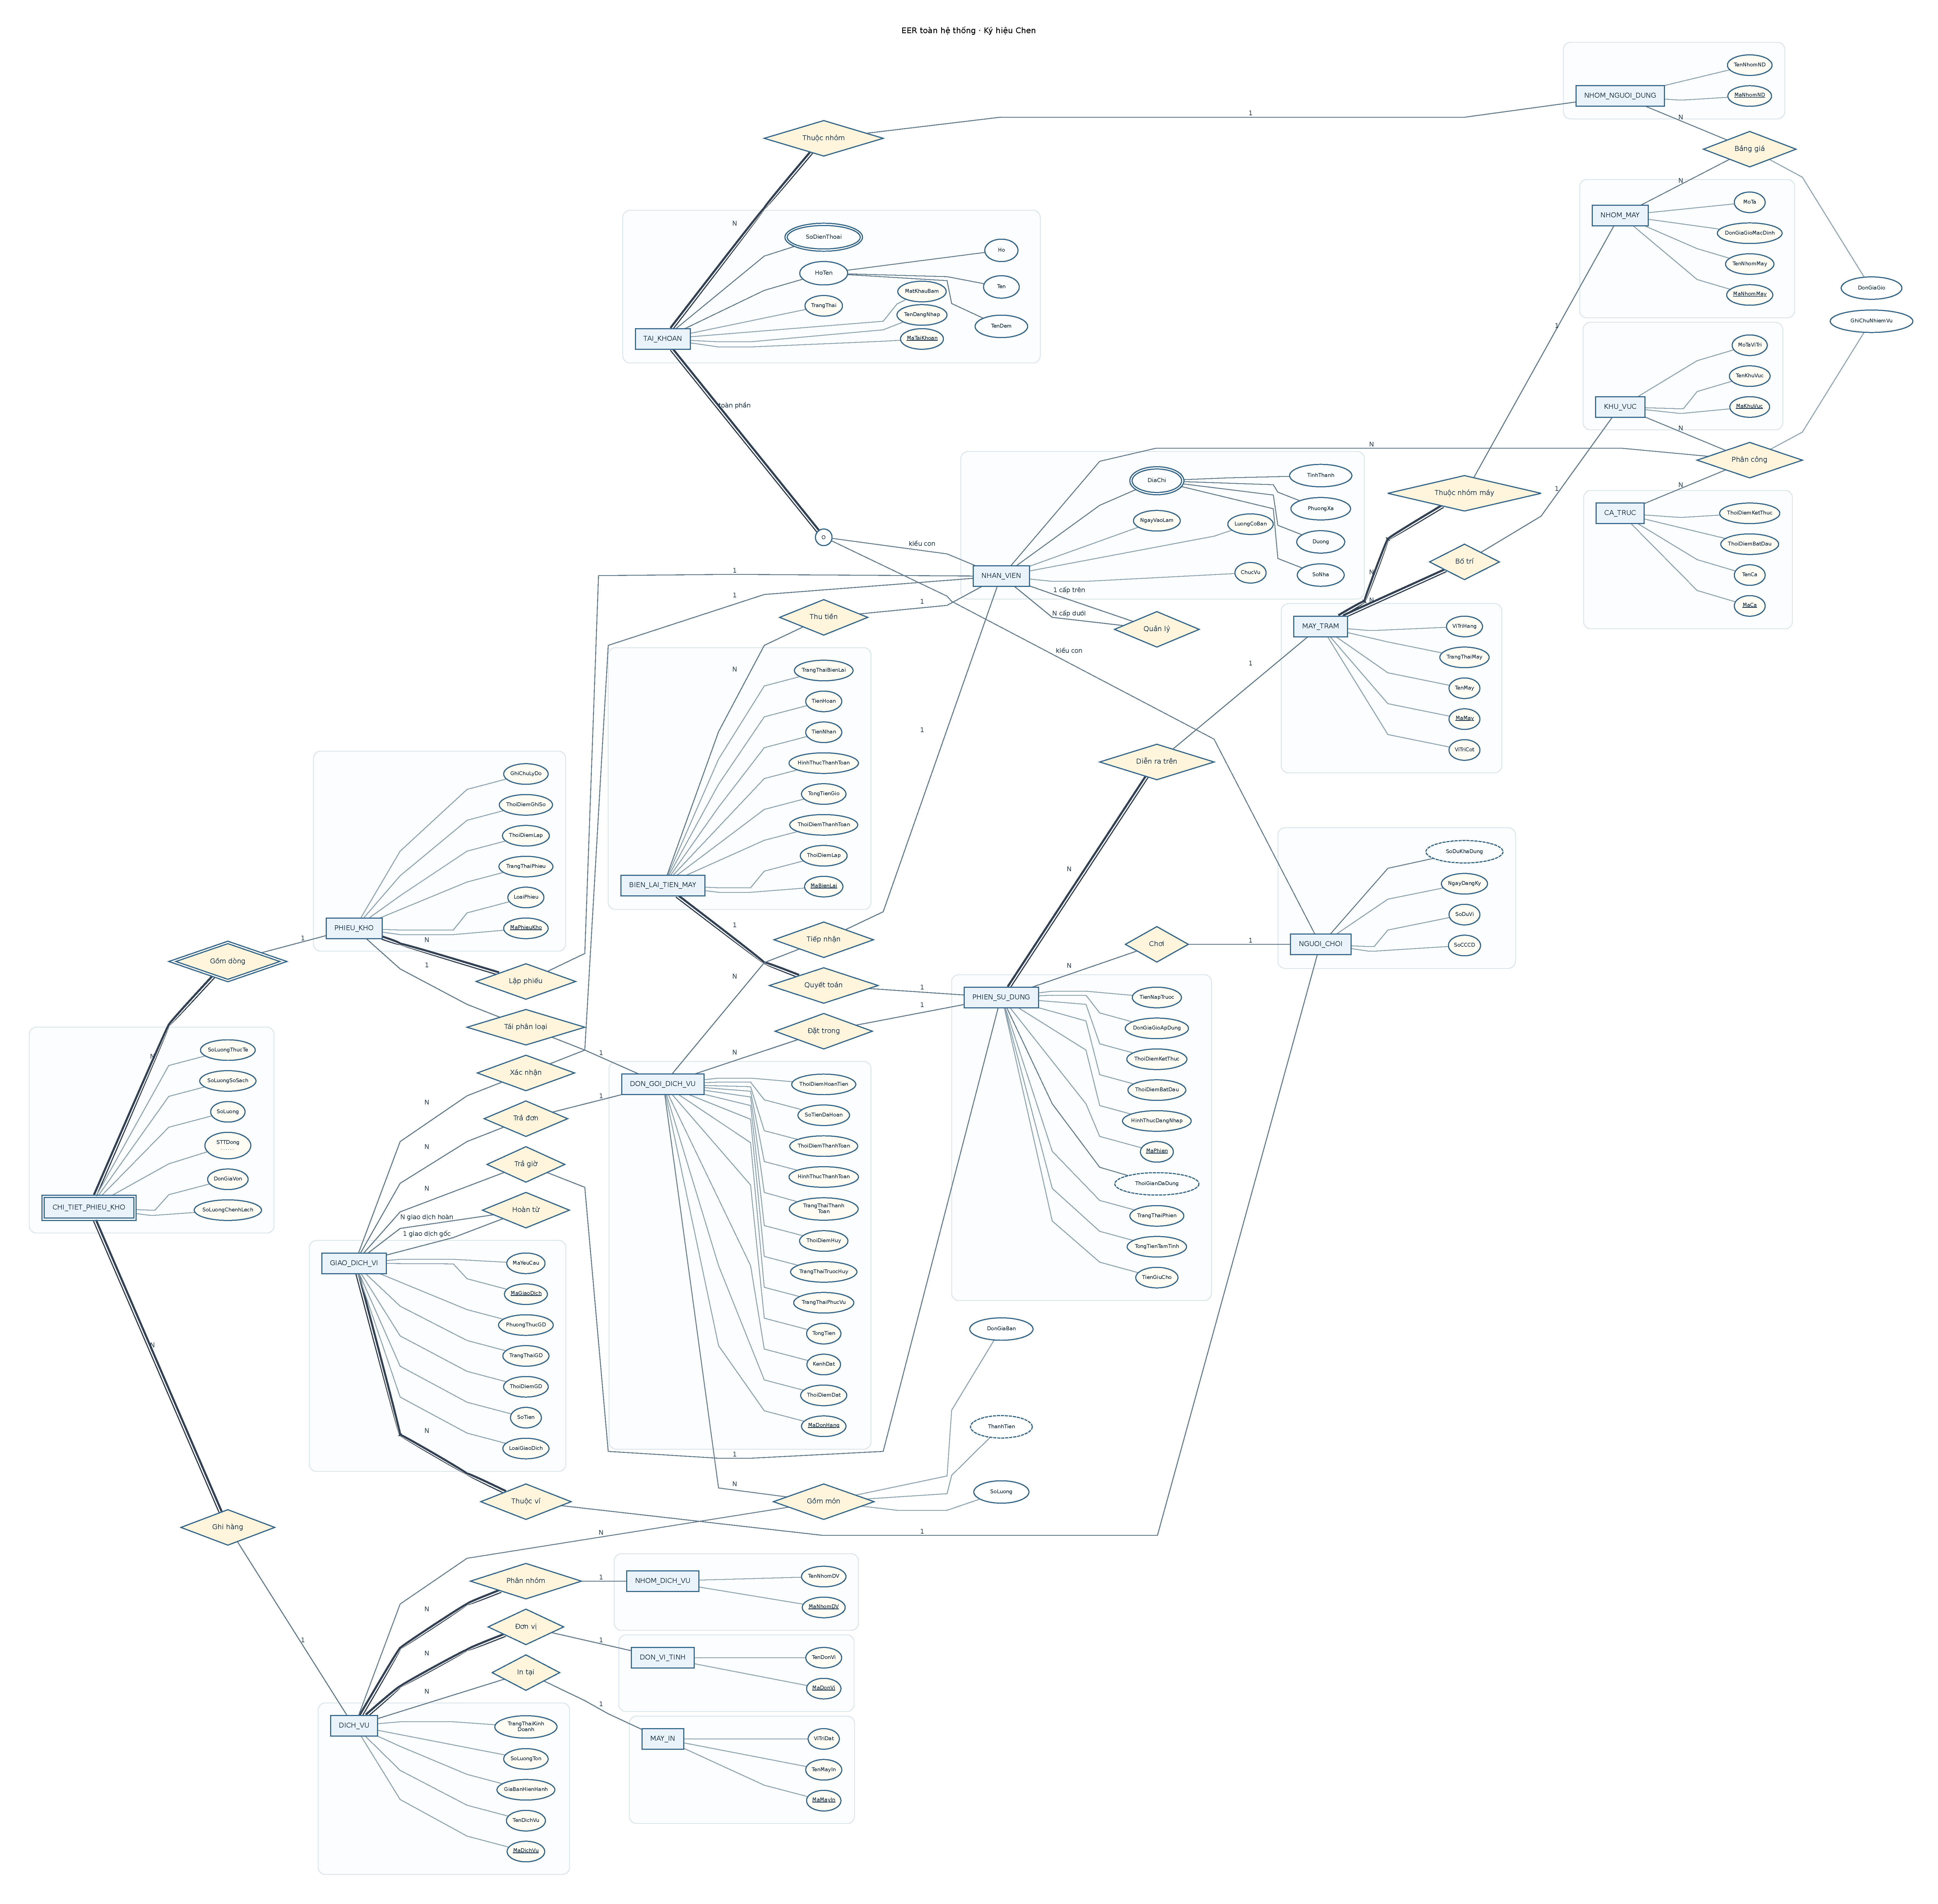
\includegraphics[width=\linewidth,height=.82\textheight,keepaspectratio]{assets/eer/erd_full_vector.pdf}\caption{Sơ đồ EER tổng thể toàn hệ thống theo ký hiệu Chen}\end{figure}
\clearpage\section{Bảng ghi chú các thay đổi so với BTL1}
\begingroup\small\setlength{\tabcolsep}{3.5pt}\renewcommand{\arraystretch}{1.2}
\begin{longtable}{@{}>{\raggedright\arraybackslash}p{28mm}>{\raggedright\arraybackslash}p{38mm}>{\raggedright\arraybackslash}p{44mm}>{\raggedright\arraybackslash}p{44mm}@{}}\toprule
\textbf{Nội dung thay đổi}&\textbf{Phiên bản cũ (BTL1)}&\textbf{Phiên bản mới (BTL2)}&\textbf{Lí do}\\\midrule\endhead
\bottomrule\endfoot
Duy nhất có điều kiện&Chỉ có ràng buộc quan hệ thực thể, chưa ràng buộc mức DBMS chống phiên mở đồng thời.&Bổ sung cột sinh và chỉ mục UNIQUE có điều kiện cho phiên đang hoạt động.&Ngăn chặn triệt để 1 tài khoản mở nhiều phiên hoặc 1 máy trạm mở cùng lúc 2 phiên.\\\midrule
Đồng bộ tổng tiền đơn&Tổng tiền đơn tính độc lập hoặc dựa vào logic tầng ứng dụng.&Bộ 3 AFTER trigger trên chi tiết dịch vụ tự động đồng bộ lại tổng tiền đầu đơn.&Bảo toàn tính nhất quán dữ liệu kế toán, không phụ thuộc ứng dụng ngoài.\\\midrule
Phân định ngày doanh thu&Thống kê doanh thu theo ngày tạo đơn hoặc ngày tạo phiên.&Tách riêng thời điểm thanh toán biên lai/đơn và thời điểm hoàn tiền.&Phản ánh đúng dòng tiền thực tế theo ngày phát sinh thay vì ngày đặt đơn.\\\midrule
Miền giá trị tiền tệ trong hàm&Dùng INT hoặc DECIMAL ngắn trong các biến tính toán của hàm.&Chuẩn hóa sang DECIMAL(18,0) cho toàn bộ biến tổng và kết quả trả về của hàm.&Tránh tràn số và sai lệch số học khi tổng tiền hoặc giao dịch ví quy mô lớn.\\\midrule
Miền chuỗi Cursor trong thủ tục&Khai báo biến tạm VARCHAR(50) ngắn trong thân thủ tục.&Khai báo khớp độ dài lược đồ (VARCHAR(100) cho tên, VARCHAR(30) cho đơn vị).&Tránh lỗi cắt cụt chuỗi dữ liệu (Data truncation) khi duyệt báo cáo tồn kho.\\\midrule
Tối ưu hóa chỉ mục thực đơn&Chỉ có các khóa chính và khóa ngoại mặc định theo thiết kế ERD.&Tạo chỉ mục phức hợp \texttt{ix\_dich\_vu\_filter} trên \texttt{(trang\_thai, ma\_nhom, ten\_dich\_vu)}.&Giảm chi phí đọc và tăng tốc truy vấn lọc thực đơn 3.88x (đo bằng EXPLAIN ANALYZE).\\\bottomrule
\end{longtable}\endgroup
\chapter{Dữ liệu mẫu và nguồn minh chứng}\label{app:data}
Mỗi hình dưới là bản xuất của SQL client trong cùng phiên kiểm chứng với các truy vấn ở Phần 1. Các dữ liệu là dữ liệu demo; không sử dụng thông tin cá nhân thật. Phần SQL và kết quả thô đầy đủ đi kèm ở thư mục evidence/dbms.
\snapshot{q01_data}{Các bảng dữ liệu mẫu liên quan Q-P12-01}{fig:q01_data}
\snapshot{q02_data}{Các bảng dữ liệu mẫu liên quan Q-P12-02}{fig:q02_data}
\snapshot{q03_data}{Các bảng dữ liệu mẫu liên quan Q-P12-03}{fig:q03_data}
\snapshot{q04_data}{Các bảng dữ liệu mẫu liên quan Q-P12-04}{fig:q04_data}
\snapshot{q05_data}{Các bảng dữ liệu mẫu liên quan Q-P12-05}{fig:q05_data}
\section{Nguồn và khả năng tái tạo}
\begin{itemize}
\item Đề gốc và mẫu Updated: thư mục \path{docs/requirements/} và tệp mẫu trong \path{docs/} của gói bàn giao.
\item DDL, khóa và routine: \path{database/01_schema/} đến \path{database/08_triggers/}.
\item Minh chứng trực tiếp: \path{evidence/dbms/manifest.json}; mỗi mục ánh xạ ảnh, câu SQL và kết quả JSON.
\item Số đo chỉ mục: \path{evidence/queries/index_benchmark.json}; kiểm thử: \path{evidence/final_verification/}.
\item Nguồn sơ đồ EER: \path{docs/btl1_baseline/BTL1_EER.drawio}; các bản vector dùng trong báo cáo nằm tại \path{assets/eer/} của bộ LaTeX.
\item Nguồn báo cáo: \path{main.tex}, các tệp \path{sections/}, \path{diagrams/} và \path{sql/}. Biên dịch bằng XeLaTeX để giữ nguyên tiếng Việt và phông chữ.
\end{itemize}

\end{document}
